本論文では,多数の人間が存在する室内空間に音源定位した複数の音を配置し用いることを考え,
音像定位を行なうシステムを開発した.
各自が所有するスマートデバイスを用いて平面配置のスピーカアレイを構築し,
所望の位置に音源配置した音声情報を提供するシステムを提案した.
この手法を用いて発生させた音は,3 つの発音端末の三角形の外の受聴者には三角形内に定位されることを確認した.
今後は,各端末の特性としてマイクやスピーカ位置,音響特性を考慮することや,端末数をどの程度まで増やすべきかの議論を行っていきたい.

\begin{figure}[p]
  \begin{center}
    \begin{tabular}{c}
      \begin{minipage}{0.3\hsize}
        \begin{center}
          \hspace{-2mm}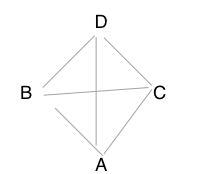
\includegraphics[clip,width=1\hsize]{img/PC_haichi.png}
          \caption{PC配置}
          \label{fig:__relpos}
        \end{center}
      \end{minipage}
      \begin{minipage}{0.68\hsize}
        \begin{center}
          \caption{50回試行時の端末間距離計測結果}
          \begin{tabular}{l|rrrrr}
            \hline
            {\footnotesize  端末間}&{\footnotesize 平均}&{\footnotesize 標準偏差}&{\footnotesize 実測距離(m) }\\
            \hline
            {\footnotesize A-D }&{\footnotesize 11.71889953}&{\footnotesize 1.24793883}&{\footnotesize 11.10 }\\
            {\footnotesize B-D }&{\footnotesize 7.767573696}&{\footnotesize 0.583510141}&{\footnotesize 7.77 }\\
            {\footnotesize C-D }&{\footnotesize 6.72675737}&{\footnotesize 0.774180135}&{\footnotesize 6.72 }\\
            {\footnotesize A-B }&{\footnotesize 6.564537924}&{\footnotesize 1.067679838}&{\footnotesize 6.83 }\\
            {\footnotesize A-C }&{\footnotesize 7.300425749}&{\footnotesize 1.283308926}&{\footnotesize 6.93 }\\
            {\footnotesize B-C }&{\footnotesize 4.771470221}&{\footnotesize 0.664454607}&{\footnotesize 4.92 }\\
            \hline
          \end{tabular}
          \label{tab:__estdistance}
        \end{center}
      \end{minipage}
    \end{tabular}
  \end{center}
\end{figure}
